\documentclass[border=4pt]{standalone}
\usepackage{amsmath,amssymb,tikz}
\usetikzlibrary{arrows.meta,calc}
\definecolor{figB}{RGB}{31,90,166}\definecolor{figR}{RGB}{176,48,48}\definecolor{figG}{RGB}{46,125,50}\definecolor{figO}{RGB}{214,120,20}
\begin{document}
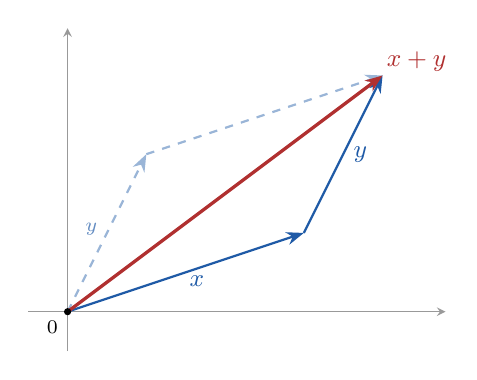
\begin{tikzpicture}[scale=1.0,>={Stealth[length=2.2mm]}]
\draw[-stealth,thin,black!40] (-0.5,0)--(4.8,0);
\draw[-stealth,thin,black!40] (0,-0.5)--(0,3.6);
% parallelogram ghosts
\draw[->,thick,figB!45,dashed] (0,0)--(1,2);
\draw[->,thick,figB!45,dashed] (1,2)--(4,3);
% tip to tail
\draw[->,thick,figB] (0,0)--(3,1) node[midway,below right,font=\small,inner sep=1pt]{$x$};
\draw[->,thick,figB] (3,1)--(4,3) node[midway,right,font=\small]{$y$};
\draw[->,very thick,figR] (0,0)--(4,3) node[above right,font=\small,inner sep=1pt]{$x+y$};
\fill (0,0) circle (1.3pt) node[below left,font=\scriptsize]{$0$};
\node[figB!70,font=\scriptsize,left] at (0.5,1.05) {$y$};
\end{tikzpicture}
\end{document}
